
\documentclass[a4j,10pt]{jsarticle}
\usepackage{layout,url,resume}
\usepackage[dvipdfmx]{graphicx}
\pagestyle{empty}

\begin{document}
%\layout

\title{SMTP Strict Transport Security (SMTP-STS)
\\を用い暗号化された電子メール通信経路の確立とその実装}

% 和文著者名
\author{
    尾崎周也 (shuya) \thanks{慶應義塾大学 総合政策学部}
    \\shuya@sfc.wide.ad.jp
    \and
    親 中島博敬 (nunnun) \thanks{慶應義塾大学 政策・メディア研究科}
    \\nunnun@sfc.wide.ad.jp
}


% 和文概要
\begin{abstract}
\\本研究ではJavaScriptでIETF UTA Working Groupで審議中であるSMTP STS(SMTP Strict Transport Security)を実装しその有用性と問題点を明らかにすることを目指す。\end{abstract}

\maketitle
\thispagestyle{empty}

\section{はじめに}

引用例\cite{example}を書いてみた.

\section{背景}

\subsection{hoge}
小見出し付きの文章.

\begin{enumerate}
\item 番号付き箇条書き 
\item 番号付き箇条書き
\end{enumerate}

\begin{itemize}
\item 箇条書き
\item 箇条書き
\end{itemize}

%---------------------------------------------

\section{研究目的}

\subsection{hoge}
hogehoge
画像を貼って見た

\begin{figure}[htbp]
    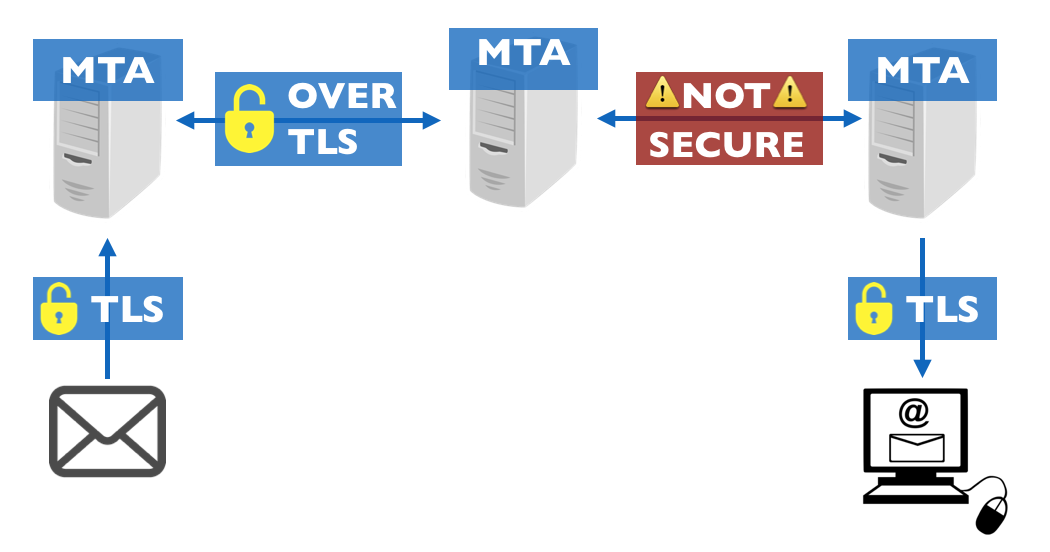
\includegraphics[width=5cm]{figure1.png}
    \caption{}
\end{figure}
 
\subsection{fuga}
fugafuga

\section{関連研究}

\section{提案手法}

\section{評価}

\section{考察}

\begin{thebibliography}{99}
%\bibitem{a}
\bibitem{example}
引用その1\\
\texttt{ http://www.example.com}
\end{thebibliography}

\end{document}
% end of file
